\subsection{Radiation and Scattering \textbf{(L9, L10)}}

\subsubsection{\hyperref[Electric Dipole Radiation]{Electric Dipole Radiation}}

Imagine two tiny metal spheres at distance $d$ from each other connected by a wire, where at time $t,$ the one sphere carries a charge $q(t)=q_{0} \cos (\omega t)$ while the other sphere is given by $-q(t)$.

\begin{enumerate}
	\item  Calculate the electric potential far away from the dipole. Use $d<<r$ and $d<<\frac{c}{\omega}$
	\item Take the limit of $\omega \rightarrow 0$ . What do you expect?
	\item Now look at the case where also $r>>\frac{c}{\omega},$ that is, when we are interested in large distances from the source in comparison to the wavelength. How does the expression for the potential simplify in this case?
	\item Obtain an expression for the vector potential in the limit $d<<r$ and $d<<$ $\frac{c}{\omega}$.
	\item Calculate the resulting electric and magnetic fields in the same limit with also $r>>\frac{c}{\omega}$.
\end{enumerate}

\subsubsection{\hyperref[Metallic Shells]{Metallic Shells}}
Two halves of a spherical metallic shell of radius $R$ and infinite conductivity are separated by a very small insulating gap. an alternating potential is applied between the two halves of the sphere so that the potentials are $\pm V$ cos $\omega t .$ In the long-wavelength limit, find the radiation field, the angular distribution of radiated power and the total radiated power from the sphere.

\subsubsection{\hyperref[Electrostatic Potential from a Dipole]{Electrostatic Potential from a Dipole}}

Consider a dipole that has distance $\vec{x}^{\prime}$ and a point $P$ at distance $\vec{x}$ far away from the dipole. Considering the general expression for the potential without boundary conditions show that at large distances from the charge distribution the potential can be approximated by using the electric dipole moment in first order. Then calculate the potential in the case where the dipole is formed by two charges $q^{+}$ and $q^{-}$ with distance $d$ between them.

\subsubsection{\hyperref[Radiation Interference]{Radiation Interference}}

Let the origin of coordinates be centered on a compact, time-harmonic source of electromagnetic radiation. The time-averaged power radiated into a differential element of solid angle $d \Omega$ centered on an observation point $\mathbf{r}$ has the form

\begin{equation}
	\frac{d P}{d \Omega} \propto|\hat{\mathbf{r}} \times \alpha|
\end{equation}

The vector $\alpha=\mathbf{p}_{0}$ if the source has a time-dependent electric dipole moment $\mathbf{p}(t)=\mathbf{p}_{0} \cos \omega t .$ The vector $\boldsymbol{\alpha}=\mathbf{m}_{0} \times \hat{\mathbf{r}}$ if the source has a time-dependent magnetic dipole moment $\mathbf{m}(t)=\mathbf{m}_{0} \cos \omega t .$ For this problem, consider a source where $\mathbf{p}(t)$ and $\mathbf{m}(t)$ are present simultaneously.

\begin{enumerate}
	\item Show that the time-averaged angular distribution of power generally exhibits interference between the two types of dipole radiation. Under what conditions is there no interference?
	\item Show that the time-averaged total power emitted by the source does not exhibit interference.
\end{enumerate}

\subsubsection{\hyperref[Sinusoidal thin Antenna]{Sinusoidal thin Antenna}}

A thin linear antenna of length $d$ is excited in such a way that the sinusoidal current makes a full wavelength of oscillation.

\begin{enumerate}
	\item Calculate exactly the power radiated per unit solid angle and plot the angular distribution of radiation.
	\item  Determine the total power radiated and find a numerical value for the radiation resistance.
	\item Calculate the multipole moments (electric dipole, magnetic dipole, and electric quadrupole) exactly.	
\end{enumerate}

\subsubsection{\hyperref[Scattering in Solid Sphere]{Scattering in Solid Sphere}}

A solid uniform sphere of radius $R$ and conductivity $\sigma$ acts as a scatterer of a plane- wave beam of unpolarized radiation of frequency $\omega,$ with $\omega R / c<<1$. The conductivity is large enough that the skin depth $\delta$ is small compared to $R$.

\begin{enumerate}
	\item Justify and use a magnetostatic scalar potential to determine the magnetic field around the sphere, assuming the conductivity is infinite.
	\item determine the absorption cross section of the sphere. Tip: The power loss from a waveguide is $\frac{P_{\text {loss }}}{d a}=\frac{1}{2 \sigma \delta}|\hat{n} \times \vec{H}|^{2}$.
\end{enumerate}

\subsubsection{\hyperref[Aperture (Science)]{Aperture (Science)}}

The aperture or apertures in a perfectly conducting plane screen can be viewed as the location of effective sources that produce radiation (the diffracted fields). An aperture whose dimensions are small compared with a wavelength acts as a source of dipole radiation with the contributions of other multipoles being negligible.

\begin{enumerate}
	\item Show that the effective electric and magnetic dipole moments can be expressed in terms of integrals of the tangential electric field in the aperture as follows:

	\begin{subequations}
		\begin{align}
			\vec{p} &=\epsilon \hat{n} \int\left(\vec{x} \cdot \vec{E}_{t a n}\right) d a, \\
			\vec{m}&= \frac{2}{i \omega \mu} \int\left(\hat{n} \times \vec{E}_{t a n}\right) d a.
		\end{align}
	\end{subequations}

	where $\vec{E}_{\text {tan }}$ is the exact tangential electric field in the aperture, $\hat{n}$ is the normal to the plane screen, directed into the region of interest, and the integration is over the area of the openings.
	\item  Show that the expression for the magnetic moment can be transformed into
	
	\begin{equation}
		\vec{m}=\frac{2}{\mu} \int \vec{x}(\hat{n} \cdot \vec{B}) d a.
	\end{equation}
\end{enumerate}

\subsubsection{\hyperref[Born Scattering from a Dielectric Cube]{Born Scattering from a Dielectric Cube}} 

A plane wave $\mathbf{E}_{0} \exp \left[i\left(\mathbf{k}_{0} \cdot \mathbf{r}-\omega t\right)\right]$ scatters from a dielectric cube with volume $V=a^{3}$ and electric susceptibility $\chi \ll 1$. Two cube edges align with $\mathbf{k}_{0}$ and $\mathbf{E}_{0}$.

\begin{enumerate}
	\item Calculate the differential scattering cross section in the Born approximation.
	\item Show that $\sigma_{\text {Born }} \approx \frac{1}{4} k^{2} a^{4} \chi^{2}$ when $k a \gg 1$. Hint: The near-forward direction dominates the scattering when $k a \gg 1$
	\item The weak scattering assumed by the Born approximation implies that 
	
	\begin{equation}
		\left|\mathbf{E}_{\mathrm{rad}}\right| /\left|\mathbf{E}_{0}\right| \ll 1,
	\end{equation}

	 for all $\mathbf{q},$ even when $r \approx a .$ Deduce from this that the $k a \gg 1$ result of part $(\mathrm{b})$ is valid only when $\sigma_{\text {Born }} \ll \chi a^{2}$.
\end{enumerate}

\subsubsection{\hyperref[E: Two Antennas Sitting Together]{E: Two Antennas Sitting Together}}

A circular loop of radius $a$ made of conducting wire is centred at the origin and lies in the $x_{3}=0$ plane. Let
be the polar angle in the $x_{3}=0$ plane (i.e. figure). The wire carries a current oscillating at frequency

\begin{equation}
	\vec{I}=I_{0} \hat{\phi} e^{-i \omega t},
\end{equation}

with $I_{0}$ real. There is also a small antenna wire of length $2a$ along $\hat{x}_{3}$ centered at the origin as in figure. An oscillating current is fed into the antenna at its midpoint so that, away from the midpoint, the wire carries a linear charge density

\begin{equation}
	\lambda=i \lambda_{0} e^{-i \omega t} ,\quad \text { for } \quad 0<x_{3}<a, \quad \lambda=-i \lambda_{0} e^{-i \omega t}+c . c, \quad \text{for} \quad -a < x_{3} < 0.
\end{equation}

Where $\lambda_{0}$ is real.

\begin{figure}[htbp!]
	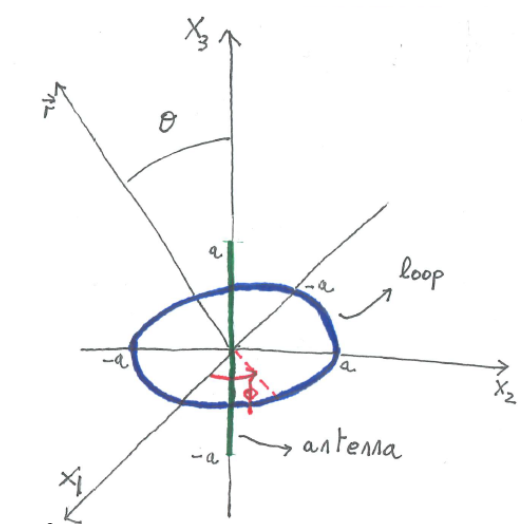
\includegraphics[width=8cm]{figures/p2examoct19.png}
	\centering
	\caption{The two described antennas.}
\end{figure}

\begin{enumerate}
	\item  Find the electric dipole moment $\vec{p}(\omega)$ and the magnetic dipole moment $\vec{m}(\omega)$ at fre-
	quency $\omega$ due to the antenna and to the wire loop.
	\item  Work in the approximation that $\frac{c}{\omega} \gg a$ so that a multipole expansion is meaningful. Determine the vector potential $\vec{A}(\vec{r}, \omega)$ in Lorentz gauge due to the dipole moments above in the radiation zone (that is $\left|\vec{r}\right| \gg \frac{c}{\omega})$.
	\item In the same approximation write down the electric and magnetic fields $\vec{E}(\vec{r}, \omega)$ and $\vec{B}(\vec{r}, \omega)$ in the radiation zone.
	\item Determine the power emitted per unit solid angle by the antenna and loop in the radiation zone. Write the answer as a function of the angle $\theta$ between $\hat{x}_{3}$ and $\hat{r}$.
\end{enumerate}

\subsubsection{\hyperref[E: One... Err, Two Antennas]{E: One... Err, Two Antennas}}

Consider a small antenna wire of length $2 a$ along $\hat{x}_{3} .$ Let the center of the wire be at the origin. A current oscillating at frequency $\omega$ is fed into the antenna at its midpoint so that away from the midpoint, the wire carries a linear charge density

\begin{equation}
	\lambda=\lambda_{0} e^{-i \omega t} \text { for } 0<x_{3}<a, \quad \lambda=-\lambda_{0} e^{-i \omega t} \quad \text { for } \quad-a<x_{3}<0,
\end{equation}

Where $\lambda_{0}$ is real.

\begin{figure}[h]
	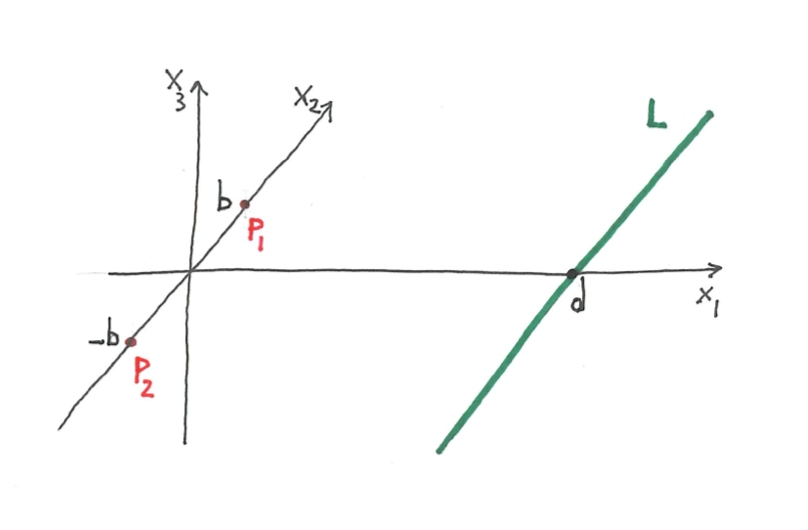
\includegraphics[width=8cm]{figures/examdec19p2.png}
	\centering
	\caption{The aforamentioned antennas.}
\end{figure}

\begin{enumerate}
	\item  Find the electric dipole moment at frequency $\omega$ of the antenna $\vec{p}(\omega)$.
	\item Determine the current $\vec{I}\left(x_{3}\right)$ flowing along the wire.
	\item Work in the approximation that $\frac{c}{\omega} \gg a$ so that a multipole expansion is meaningful. Determine the vector potential $\vec{A}(\vec{r}, \omega)$ in Lorentz gauge due to the antenna in the radiation zone (that) is $\left.|\vec{r}| \gg \frac{c}{\omega}\right)$.
	\item In the same approximation write down the electric and magnetic fields $\vec{E}(\vec{r}, \omega)$ and $\vec{B}(\vec{r}, \omega)$ in the radiation zone.
	\item Now consider placing two antennas identical to the one above at the two points (see figure)
	
	\begin{equation}
		P 1:\left(x_{1}=0, x_{2}=b, x_{3}=0\right) \text { and } \mathrm{P} 2:\left(\mathrm{x}_{1}=0, \mathrm{x}_{2}=-\mathrm{b}, \mathrm{x}_{3}=0\right).
	\end{equation}

	The two antennas are pointing along $\hat{x}_{3}$ and they are oscillating in phase.

	\begin{enumerate}
		\item Let $b=\frac{5 \pi c}{\omega} .$ Determine the electric field $\vec{E}\left(x_{2}\right)$ along the line $L$ (see figure) located at $x_{3}=0, x_{1}=d .$ Assume that $d \gg b$
		\item Does the electric field you found above vanish somewhere along the line $L ?$ If so where?
		Explain your result.
	\end{enumerate}
\end{enumerate}
	
	
\subsubsection{\hyperref[E : Who bent my Antenna?]{E : Who bent my Antenna?}}
	
An antenna is made of a circular conducting wire loop of radius $a$ centered at the origin. It lies in the $x=0$ plane. Let $-\pi<\alpha \leq \pi$ be the polar angle in the $x=0$ plane (see figure at the top of next page). There is a gap in the wire at $\alpha=\pi$ so no current can flow across. The antenna is fed an RF signal at $\alpha=0$ so that the wire carries a current oscillating at frequency $\omega$

\begin{equation}
		\vec{I}=I_{0}(\pi-|\alpha|) \hat{\alpha} e^{-i \omega t}, \quad-\pi<\alpha<\pi,
\end{equation}

with $I_{0}$ real.
	
\begin{figure}[h]
	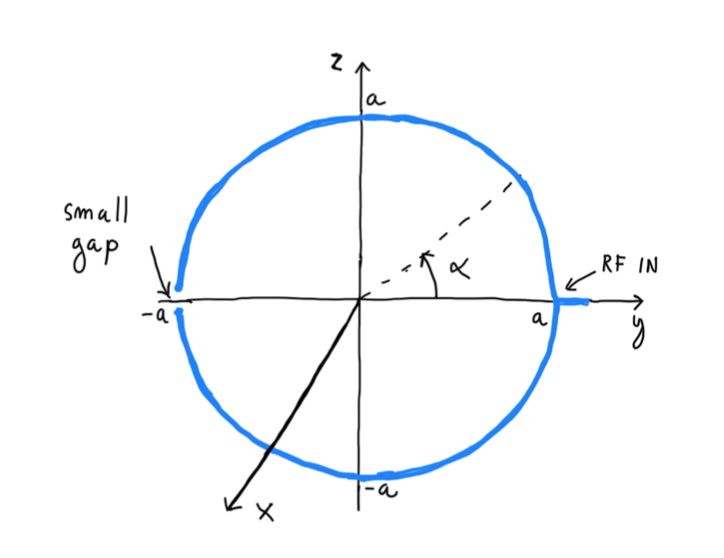
\includegraphics[width=8cm]{figures/examoct20p3.png}
	\centering
	\caption{Who bent it?}
\end{figure}

\begin{enumerate}
	\item Find the electric dipole moment $\vec{p}(\omega)$ and the magnetic dipole moment $\vec{m}(\omega)$ at frequency $\omega$ of the wire loop.
	\item Work in the approximation that $\frac{c}{\omega} \gg a$ so that a multipole expansion is meaningful. Determine the vector potential $\vec{A}(\vec{r}, \omega)$ in Lorentz gauge in the radiation zone (that is $\left|\vec{r}\right| \gg \frac{c}{\omega})$ due to the dipole moments above.
	\item In the same approximation write down the electric and magnetic fields $\vec{E}(\vec{r}, \omega)$ and $\vec{B}(\vec{r}, \omega)$ in the radiation zone.
	\item Determine the power emitted per unit solid angle by the loop in the radiation zone.
\end{enumerate}
	
